%This work is licensed under Creative Commons Attribution-NonCommercial-ShareAlike 4.0 International. To view a copy of this license, visit https://creativecommons.org/licenses/by-nc-sa/4.0

\documentclass[12pt]{exam}
\newcommand{\semanticversion}{v2.1.0}               % Release version
\newcommand{\studentone}{Gage Linville}			    % Enter your name
\title{Diaprepes Root Weevil Texas Quarantine Reference}			    % Title of the project
\newcommand{\creationdate}{April 11th, 2025}         % Creation date
\newcommand{\revisiondate}{May 24th, 2025}           % Revision date
							
%-------------------------------------------------------------------------------------
%  PACKAGES
%-------------------------------------------------------------------------------------
\usepackage{graphicx}	
\usepackage{fourier} % Font file
\usepackage{titlesec} % Package that allows for a period to be placed after a section number

%-------------------------------------------------------------------------------------
%  GRAPHICS PATH
%-------------------------------------------------------------------------------------
\graphicspath{{figures/}}					      % Put your figures in a folder called figures

%-------------------------------------------------------------------------------------
% FUNCTIONS FOR IMPORTING FIGURES
%-------------------------------------------------------------------------------------
\newcommand{\placefigure}[1]{\centerline{\includegraphics[width=2 in]{#1}}} 
\newcommand{\placefigureandscale}[2]{\centerline{\includegraphics[width=#2 in]{#1}}} 

%-------------------------------------------------------------------------------------
% ADDITIONAL COMMANDS
%-------------------------------------------------------------------------------------
\renewcommand{\labelenumi}{\alph{enumi})}
\titlelabel{\thetitle.\quad} % Function for executing period after section number
%-------------------------------------------------------------------------------------
% TITLE PAGE MACRO
%-------------------------------------------------------------------------------------
\makeatletter
\def\maketitle{%
  \null
  \thispagestyle{empty}
  \begin{center}\leavevmode
       \normalfont
       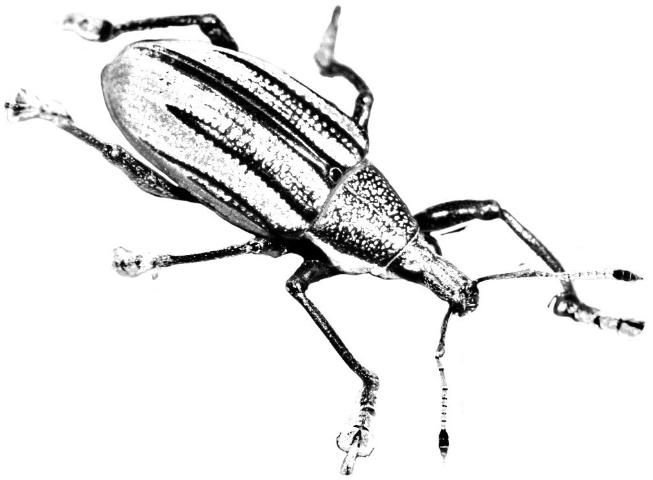
\includegraphics[width=0.20\columnwidth]{figures/Image.png}
	\rule{\linewidth}{0.2 mm} \\[0.4 cm]
	{ \huge \bfseries \@title}\\
	\rule{\linewidth}{0.2 mm} \\[0.4 cm]

	\begin{minipage}{0.5\textwidth}
		 \begin{center}\large
			Compiled by: \studentone\\
            Created: \creationdate\\
            Revised: \revisiondate\\
            \semanticversion\\
            \
			\end{center}
			\end{minipage}
   \end{center}
   \vfill
   \null
   \cleardoublepage
  }
\makeatother

%-------------------------------------------------------------------------------------
% START OF DOCUMENT
%-------------------------------------------------------------------------------------

\begin{document}
%\large 
\maketitle
%\frontmatter
\let\cleardoublepage\clearpage
%\mainmatter
\sloppy

%-------------------------------------------------------------------------------------
% CONTENTS
%-------------------------------------------------------------------------------------
\section*{Quarantined Pest:}
The quarantined pest is the Diaprepes root weevil, \textit{Diaprepes abbreviatus} in any living stage of development. 

\section*{Quarantine Regulations:}
The Texas Department of Agriculture's Diaprepes root weevil quarantine regulations are found in the Texas Admin Code: Title 4, Chapter 19, Subchapter P, Rule §§19.160-19.163.

\section*{Quarantined Articles:}
\begin{enumerate}
\item The quarantined pest.
\item Soil, sand, or gravel separately or combined with other potting media.
\item All propagation material including all plants and plant parts.
\item Citrus plants and all other plants capable of hosting the quarantined pest.
\item All nursery stock and field grown ornamentals that are potted or balled and burlaped
\end{enumerate}

\section*{Geographic Areas Subject to Quarantine:}

\section{Outside Texas:}

\begin{enumerate}
\item The following counties in the State of Florida: Broward, Collier, Miami-Dade, DeSoto, Glades, Hendry, Highlands, Hillsborough, Indian River, Lake, Lee, Manatee, Marion, Martin, Orange, Osceola, Palm Beach, Pasco, Polk, Seminole, St. Lucie, Sumter, and Volusia.
\item Commonwealth of Puerto Rico.
\item The island of the West Indies.
\item Any other area where this pest is detected.
\end{enumerate}

\section{Within Texas:}
\begin{enumerate}
\item Cameron, Harris, and Hidalgo County. The quarantine only applies to specific areas within these counties, and those may be viewed on the Texas Department of Agriculture's website. It is not specified in the Texas Admin Code.
\end{enumerate}
\newpage
\section*{Major Host Crops of \textit{Diaprepes abbreviatus}:} %Figure out how to italicize this
\begin{center}
\begin{tabular}{ |c|c| } 
 \hline
 \textbf{Common Name} & \textbf{Scientific Name }\\ 
 \hline
 Aloe & \textit{Aloe vera} \\ 
 \hline
 Bean & \textit{Phaseolus sp.} \\ 
 \hline
 Corn & \textit{Zea mays} \\ 
 \hline
 Cotton & \textit{Gossypium spp.} \\
 \hline
 Eggplant & \textit{Solanum melongena} \\ 
 \hline
 Grapefruit & \textit{Citrus x paradisi} \\ 
 \hline
 Lemon & \textit{Citrus x limon} \\ 
 \hline
 Lime & \textit{Citrus x aurantifolia} \\ 
 \hline
 Okra & \textit{Abelmoschus esculentus} \\
 \hline
 Orange & \textit{Citrus x sinensis} \\ 
 \hline
 Pea & \textit{Cajanus cajan} \\ 
 \hline
 Peach & \textit{Prunus persica} \\
 \hline
 Peanut & \textit{Arachis hypogaea} \\
 \hline
 Pecan & \textit{Carya illinoinensis} \\
 \hline
 Pepper & \textit{Capsicum annuum} \\
 \hline
 Potatoe & \textit{Solanum tuberosum} \\
 \hline
 Sorghum & \textit{Sorghum bicolor} \\
 \hline
 Bitter Orange & \textit{Citrus aurantium} \\ %This is also commonly called the "sour orange" https://en.wikipedia.org/wiki/Bitter_orange
 \hline
 Sugarcane & \textit{Saccharum officinarum} \\
 \hline
 Sweet Potatoe & \textit{Ipomoea batatas} \\
 \hline
 Tangerine & \textit{Citrus reticulata} \\ %There's more nuance to this. Targerines are considered to be a variety of mandrine orange.
 \hline
 Tobacco & \textit{Nicotiana tabacum} \\
 \hline
 Yam & \textit{Dioscorea batatas} \\
 \hline
\end{tabular}
\end{center}
\vspace{0.2in}

\textbf{References:}\\
1. TDA Website: https://texasagriculture.gov/Regulatory-Programs/Plant-Quality/Pest-and-Disease-Alerts/Diaprepes-Root-Weevil
% Texas Admin Code Direct Link: https://texas-sos.appianportalsgov.com/rules-and-meetingscchapter=19&interface=VIEW_TAC&part=1&subchapter=P&title=4 

\end{document}